\documentclass[]{beamer}
% Class options include: notes, notesonly, handout, trans,
%                        hidesubsections, shadesubsections,
%                        inrow, blue, red, grey, brown

% Theme for beamer presentation.
\usepackage{beamerthemesplit} 



%%%%%%%%%%%%%%%%%%%%%%%%%%%%%%%%%%%%%%%%%%%%%%%%%%%%%%%%%%%%%%%%%%%%%%



\definecolor{mypink1}{rgb}{0.858, 0.188, 0.478}

\newcommand{\mybox}{%
    \collectbox{%
        \setlength{\fboxsep}{1pt}%
        \fbox{\BOXCONTENT}%
    }%
}

%%%%%%%%%%%%%%%%%%%%%%%%%%%%%%%%%%%%%%%%%%%%%%%%%%%%%%%%%%%%%%%%%%%%%%
% Other themes include: beamerthemebars, beamerthemelined, 
%                       beamerthemetree, beamerthemetreebars  

\title{PHY250: Waves}    % Enter your title between curly braces
\author{Anabela R. Turlione}                 % Enter your name between curly braces
\institute{Digipen}      % Enter your institute name between curly braces
\date{Fall 2021}                    % Enter the date or \today between curly braces


\begin{document}

% Creates title page of slide show using above information
\begin{frame}
  \titlepage
\end{frame}
%\note{Talk for 30 minutes} % Add notes to yourself that will be displayed when
                           % typeset with the notes or notesonly class options

\section[]{}

% Creates table of contents slide incorporating
% all \section and \subsection commands
\begin{frame}
  \tableofcontents
\end{frame}


% \begin{frame}
%   % \centering
%    \movie[externalviewer]{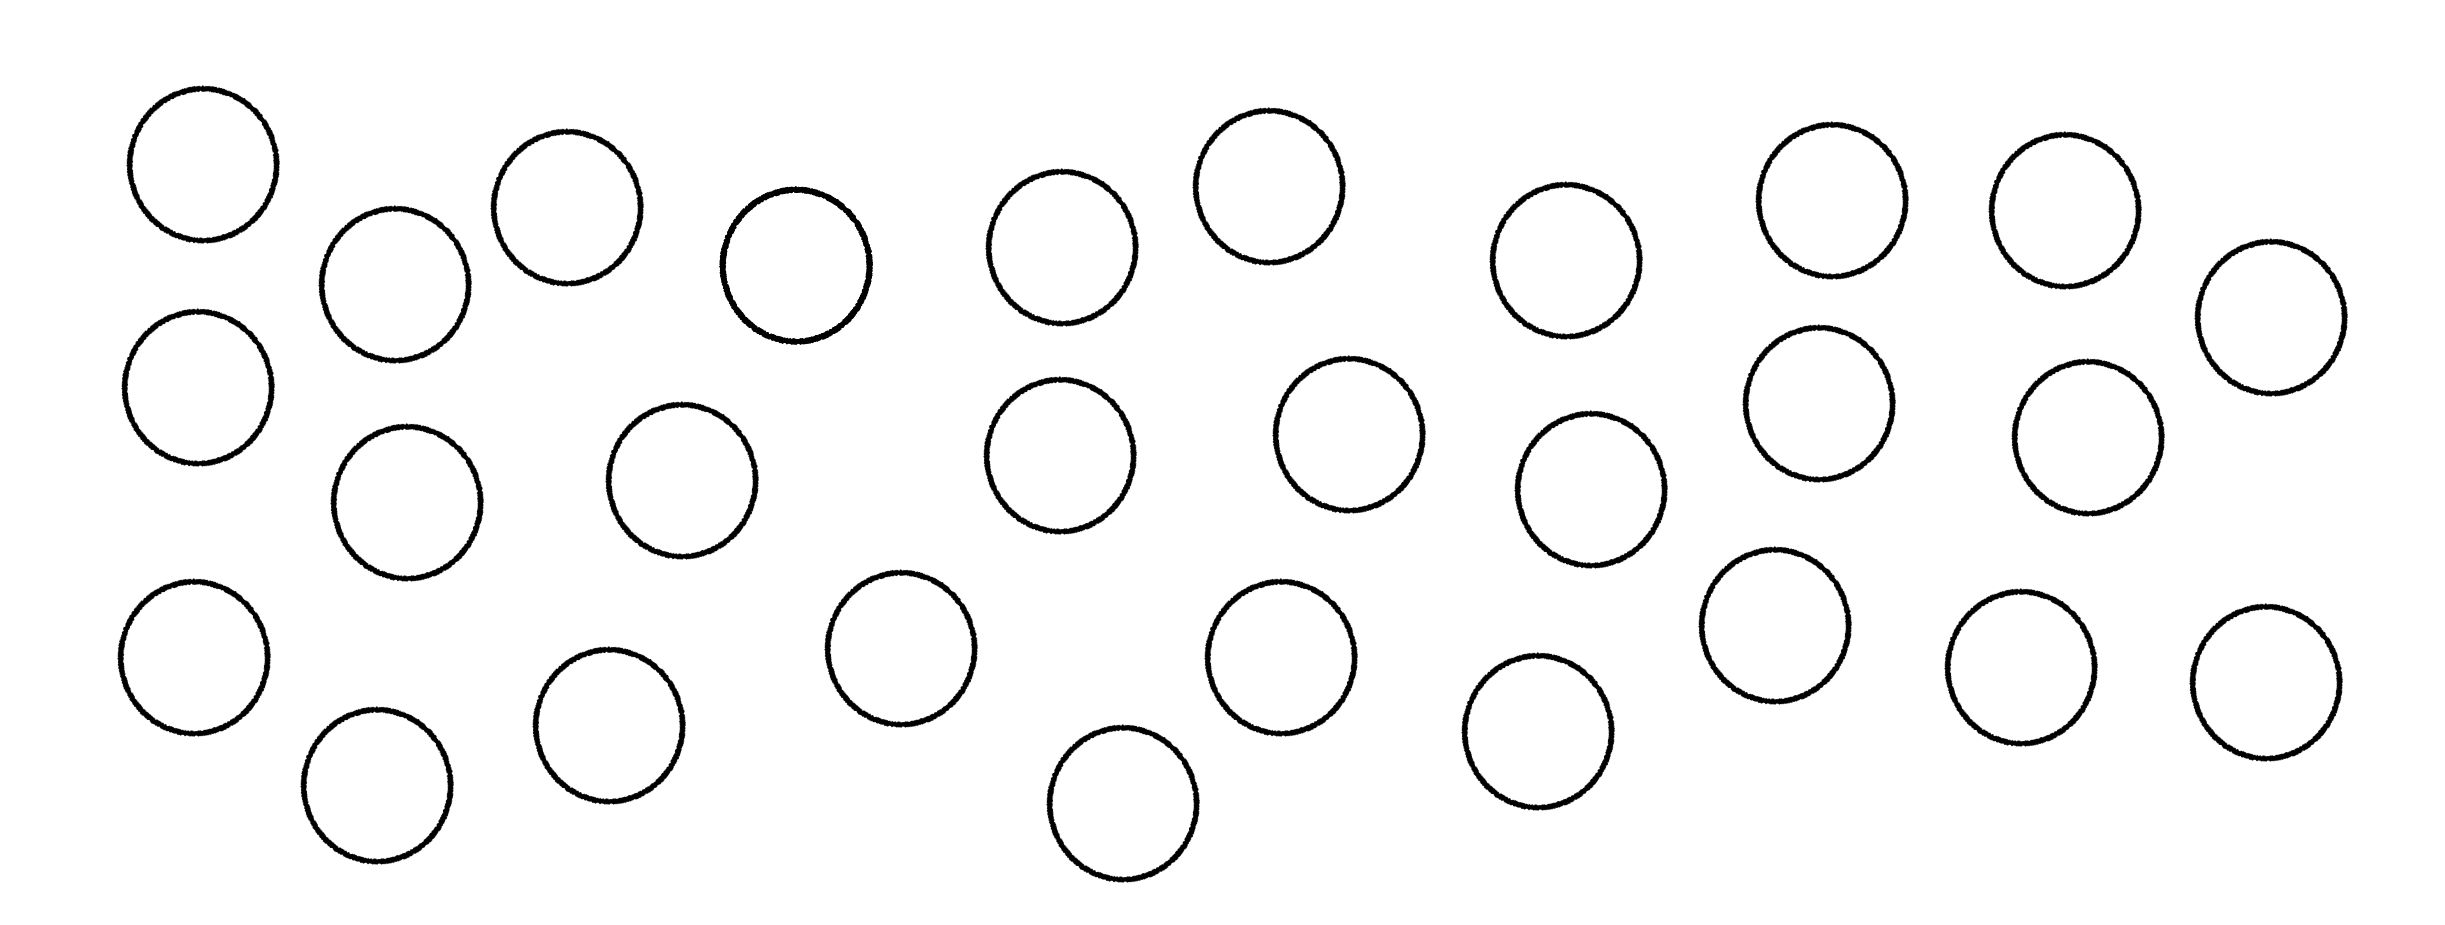
\includegraphics[width=\textheight ,
%    keepaspectratio]{surfacet1.jpg}}{test.mp4}

% \end{frame}
%%%%%%%%%%%%%%%%%%%%%%%%%%%%%%%%%%%%%%%%%%%%%%%%%%%%%%%%%%%%%%%%%%%

%%%%%%%%%%%%%%%%%%%%%%%%%%%%%%%%%%%%%%%%%%%%%%%%%%%%%%%%%%%%%%%%%%%
\section{Wave Motion}

\begin{frame}
\frametitle{Itroduction}

So far we have studied the Simple Harmonic Motion of a single particle...

\begin{center}
  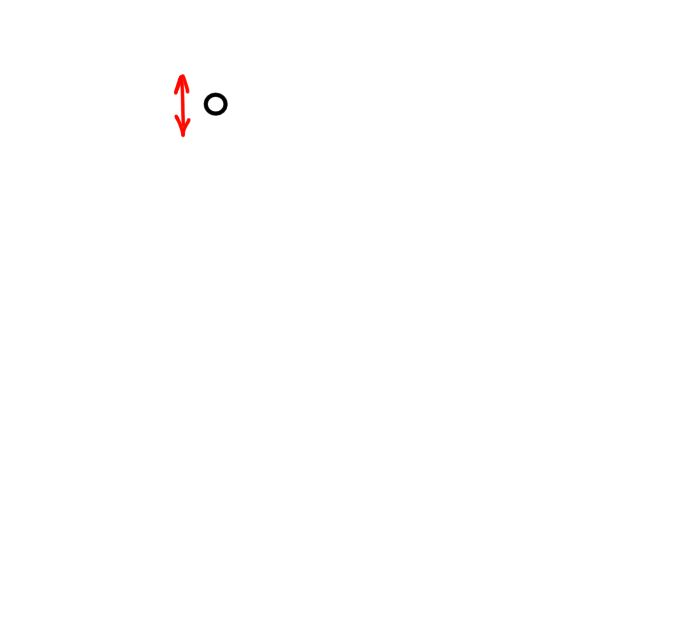
\includegraphics[height=2.2in]{images4/0b.jpg}
\end{center}

  \end{frame}

%%%%%%%%%%%%%%%%%%%%%%%%%%%%%%%%%%%%%%%%%%%%%%%%%%%%%%%%%%%%%%%%%%%


\begin{frame}
\frametitle{Introduction}

What happens if the the particle that is oscillating is part of a medium? 

\begin{center}
  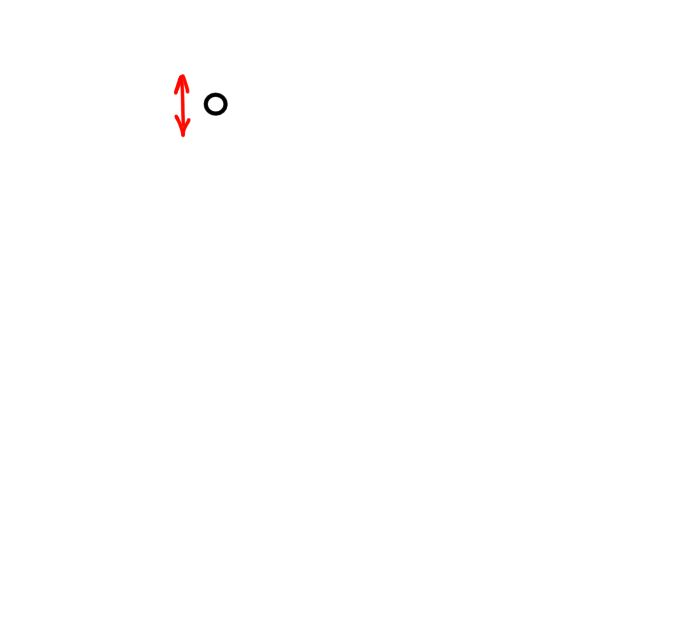
\includegraphics[height=2.2in]{images4/0b.jpg}
\end{center}

  \end{frame}
%%%%%%%%%%%%%%%%%%%%%%%%%%%%%%%%%%%%%%%%%%%%%%%%%%%%%%%%%%%%%%%%%%%


\begin{frame}
\frametitle{Introduction}

What happens if the the particle that is oscillating is part of a medium? 

\begin{center}
  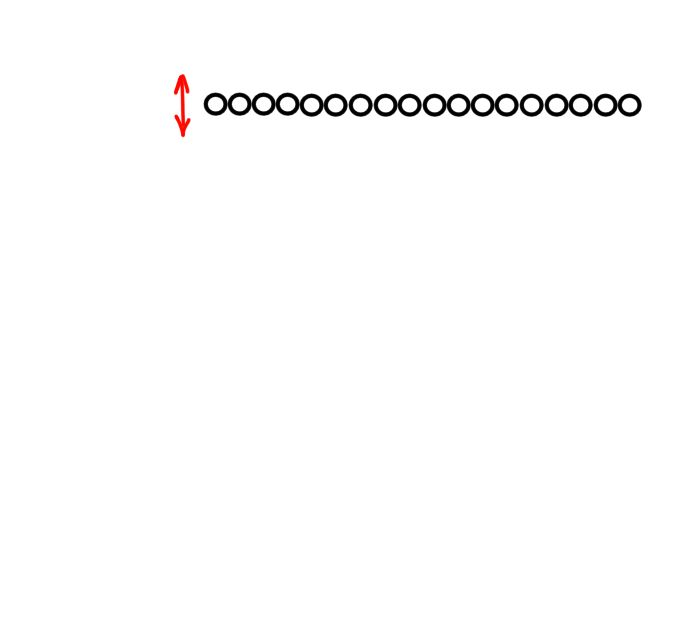
\includegraphics[height=2.2in]{images4/0c.jpg}
\end{center}

  \end{frame}

%%%%%%%%%%%%%%%%%%%%%%%%%%%%%%%%%%%%%%%%%%%%%%%%%%%%%%%%%%%%%%%%%%%
\begin{frame}
\frametitle{Introduction}

What happens if the the particle that is oscillating is part of a medium? 

\begin{center}
  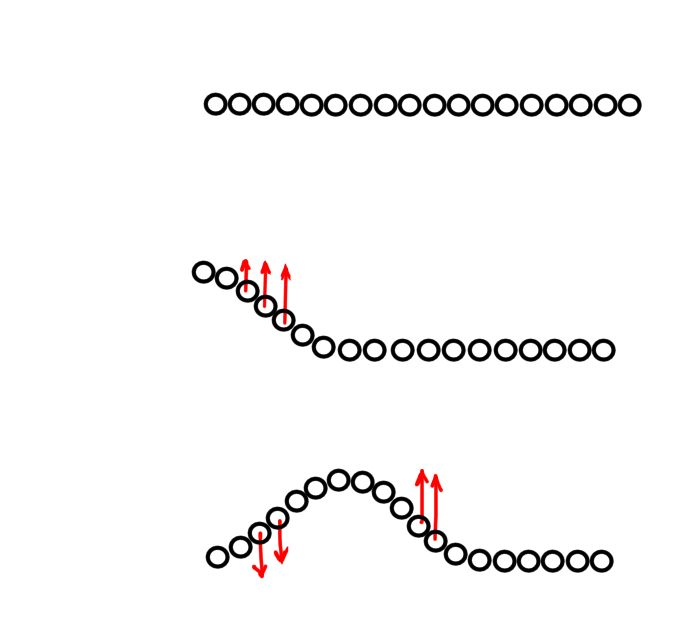
\includegraphics[height=2.2in]{images4/0.jpg}
\end{center}

  \end{frame}

%%%%%%%%%%%%%%%%%%%%%%%%%%%%%%%%%%%%%%%%%%%%%%%%%%%%%%%%%%%%%%%%%%%


\begin{frame}
\frametitle{Mechanical Waves}

A wave consists of oscillations that moves without carrying matter with them. Examples:
\vspace{3mm}

\pause

\begin{itemize}
\item Sound waves
\pause
\item Waves on a cord
\pause
\item Water waves
\end{itemize}




  \end{frame}

  %%%%%%%%%%%%%%%%%%%%%%%%%%%%%%%%%%%%%%%%%%%%%%%%%%%%%%%%%%%%%%%%%%%


\begin{frame}
  \frametitle{Mechanical Waves}
  

  
  \begin{itemize}
    \item \textcolor{mypink1}{The waves move with a recognizable velocity} \pause
    \item \textcolor{mypink1}{Each particle oscillates about an equilibrium position}\pause
    \item \textcolor{mypink1}{Waves can move over large distances,  the medium   has only a limited motion. }\pause
    \item \textcolor{mypink1}{Mechanical Waves carry  Energy as oscillation of matter, they does not carry matter.}
  \end{itemize}
  
  
 
  
  
  
  
    \end{frame}
%%%%%%%%%%%%%%%%%%%%%%%%%%%%%%%%%%%%%%%%%%%%%%%%%%%%%%%%%%%%%%%%%%%

\begin{frame}
\frametitle{Mechanical Waves}

Example: How a wave is formed in a cord?
\vspace{5mm}

\pause


   \begin{columns}[c]
   \column{2in}  % slides are 3in high by 5in wide
  
\begin{center}
  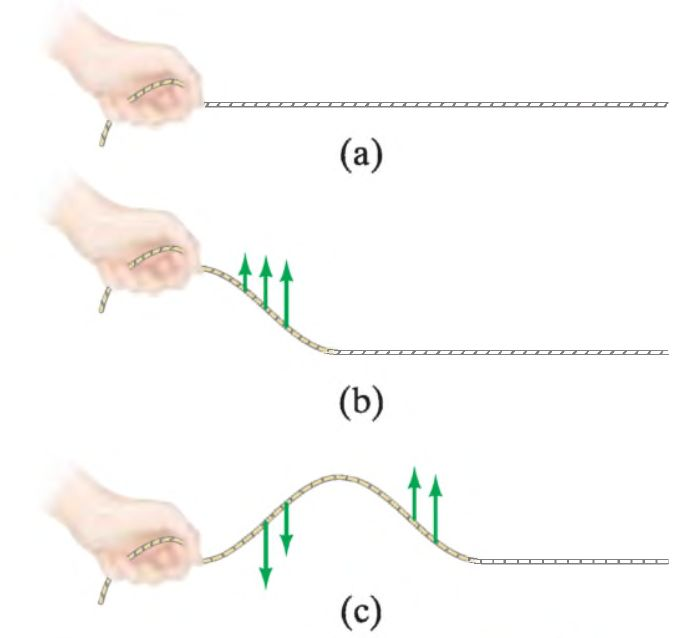
\includegraphics[height=1.7in]{images4/1.jpg}
\end{center}
\pause
   \column{2in}
Single pulse formation: The hand pulls up and down on one end of the cord, each section of the cord is pulled up and down by the tension made by the adjacent section.
The source of the traveling wave pulse is a disturbance, and cohesive forces between adjacent section of the cord cause the pulse to travel.
   \end{columns}






  \end{frame}
%%%%%%%%%%%%%%%%%%%%%%%%%%%%%%%%%%%%%%%%%%%%%%%%%%%%%%%%%%%%%%%%%%%
\begin{frame}
\frametitle{Mechanical Waves}


Source vibrates sinusoidally in a SHM $\rightarrow$ The wave itself will have a sinusoidal shape that depends on both,  time and space. 
\pause
\vspace{5mm}

\begin{enumerate}
\item In space: If you take a picture of the wave at a given instant of time, the wave will have the shape of a sine or a cosine.
\pause
\item In time: the up-down motion of  an small segment  of  the cord at a certain position will be Simple Harmonic Motion.

\end{enumerate}

  \end{frame}

%%%%%%%%%%%%%%%%%%%%%%%%%%%%%%%%%%%%%%%%%%%%%%%%%%%%%%%%%%%%%%%%%%%
\begin{frame}
\frametitle{Periodic Sinusoidal Waves}



Picture of the wave at a certain time:
\pause

\vspace{5mm}

  \begin{center}
  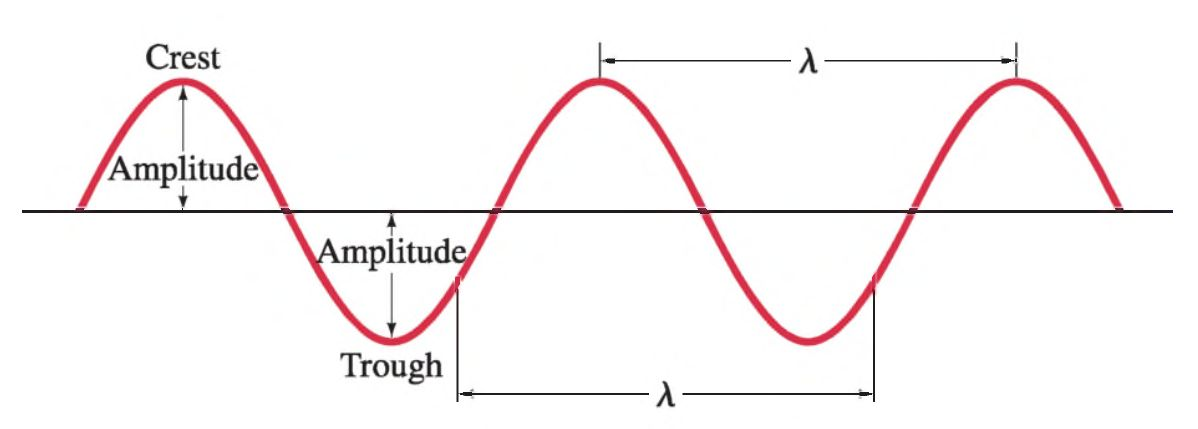
\includegraphics[height=1.3in]{images4/2.jpg}
\end{center}
\pause
The \textbf{wave velocity}, $v$, is the velocity at which wave crests move forward. 
\pause
\begin{equation}
\boxed{v=\lambda /T=\lambda f}
\end{equation}

  \end{frame}

%%%%%%%%%%%%%%%%%%%%%%%%%%%%%%%%%%%%%%%%%%%%%%%%%%%%%%%%%%%%%%%%%%%
\begin{frame}
\frametitle{Types of waves}
\pause
 \begin{itemize}
\item \textcolor{mypink1}{\textbf{Transverse waves}} The vibration up-down  of the particles of the medium are in a direction transverse to the motion of the wave itself.
\pause
\item \textcolor{mypink1}{\textbf{Logitudinal Waves}} The vibration of the particles in the medium is along the direction of the wave's motion.
\pause
\end{itemize}

\pause

 \begin{center}
  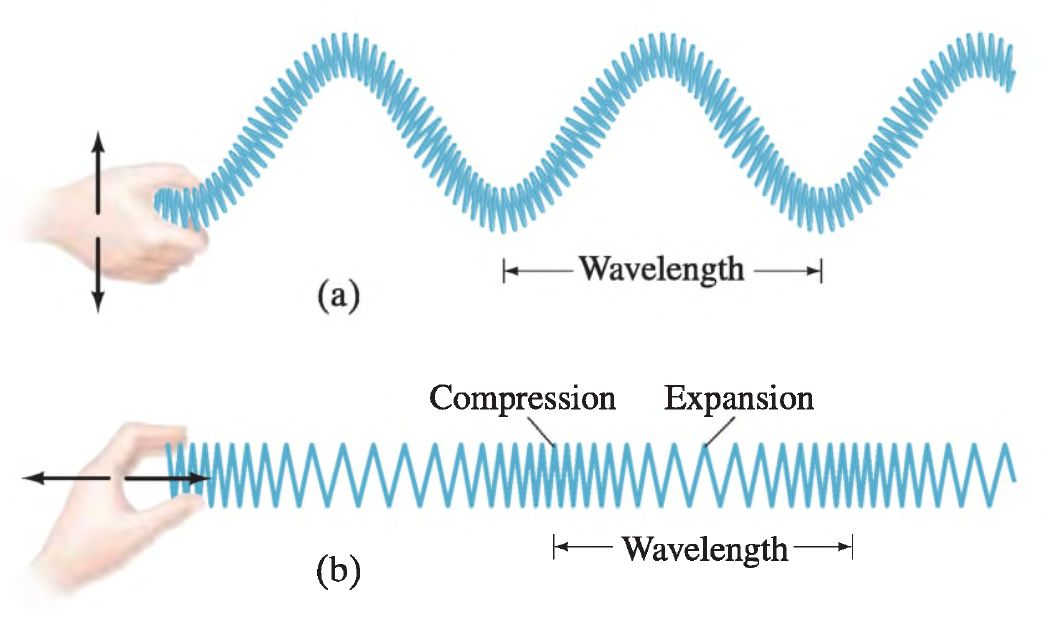
\includegraphics[height=1.5in]{images4/3.jpg}
\end{center}

\end{frame}




%%%%%%%%%%%%%%%%%%%%%%%%%%%%%%%%%%%%%%%%%%%%%%%%%%%%%%%%%%%%%%%%%%%
\begin{frame}
\frametitle{Types of waves}

Sound waves: example of longitudinal waves.
\pause

\vspace{5mm}

 A vibrating drumhead, for instance, alternately compresses and rarefies the air in contact with it,
producing a longitudinal wave that travels outward in the air. 
\pause
 \begin{center}
  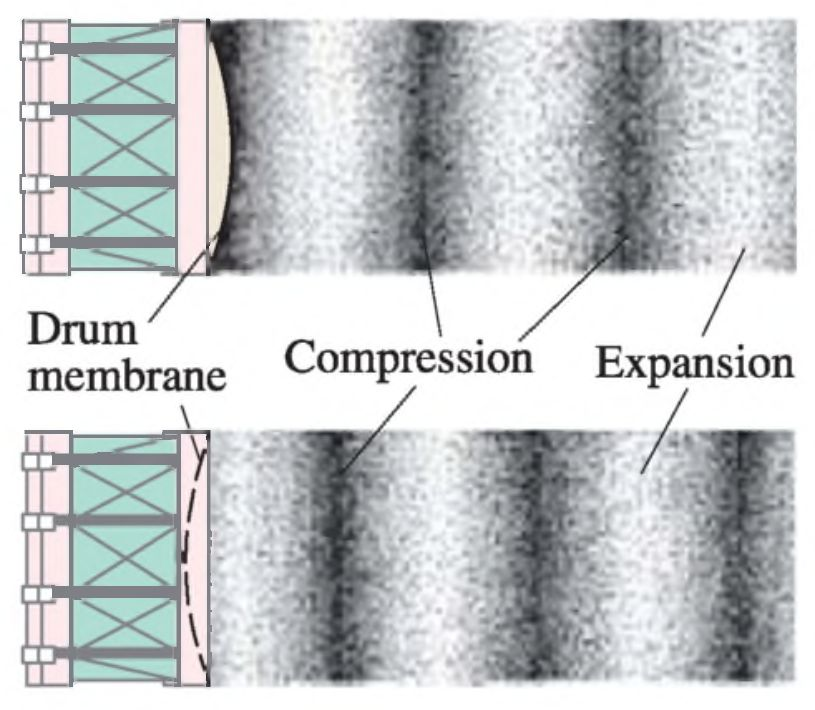
\includegraphics[height=1.5in]{images4/5.jpg}
\end{center}

  \end{frame}


%%%%%%%%%%%%%%%%%%%%%%%%%%%%%%%%%%%%%%%%%%%%%%%%%%%%%%%%%%%%%%%%%%%
\begin{frame}
\frametitle{Types of waves}

A longitudinal wave can be represented graphically by plotting the density of
air molecules versus position at a given instant.
\pause

 \begin{center}
  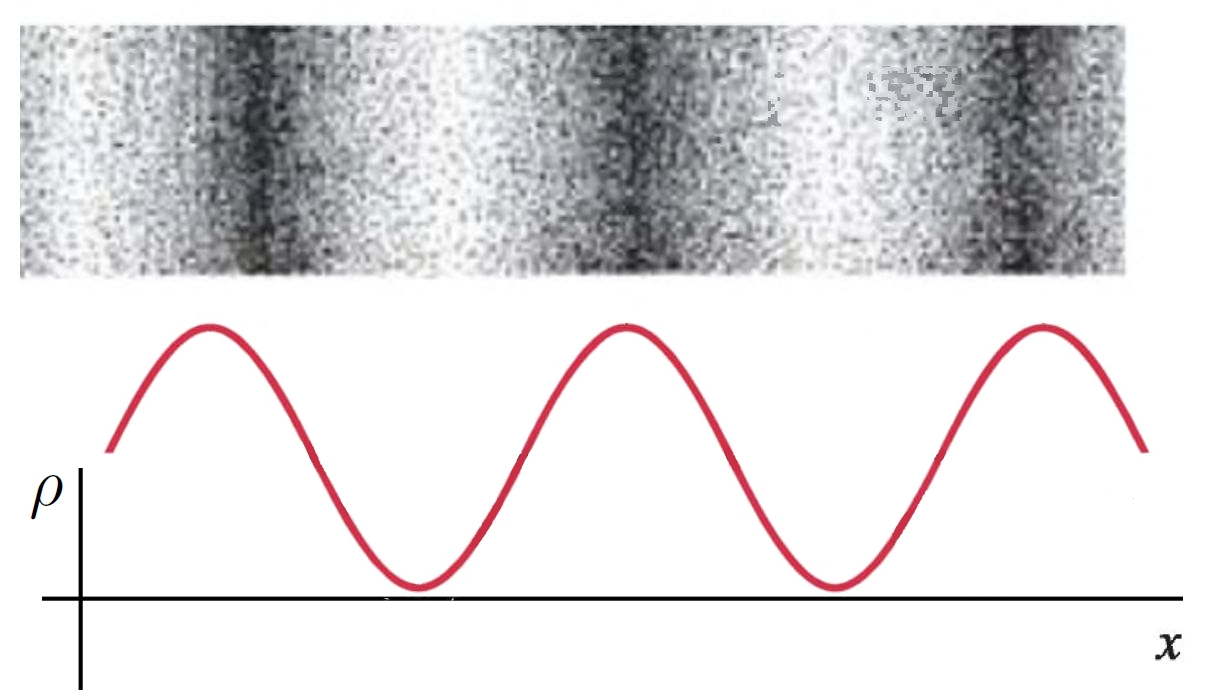
\includegraphics[height=1.5in]{images4/4.jpg}
\end{center}

  \end{frame}



%%%%%%%%%%%%%%%%%%%%%%%%%%%%%%%%%%%%%%%%%%%%%%%%%%%%%%%%%%%%%%%%%%%
\begin{frame}
\frametitle{Speed of transverse Waves}
The velocity of a wave depends on the properties of the medium in which it travels.
\pause

\begin{equation}
v=\sqrt{\frac{F_T}{\mu}}
\end{equation}
\pause

where, $F_T$ is the tension on the cord and $\mu$ is the longitudinal density.


  \end{frame}

%%%%%%%%%%%%%%%%%%%%%%%%%%%%%%%%%%%%%%%%%%%%%%%%%%%%%%%%%%%%%%%%%%%
\begin{frame}

\textcolor{mypink1}{Proof:}




   \begin{columns}[c]
   \column{2.5in}  % slides are 3in high by 5in wide

 \begin{center}
  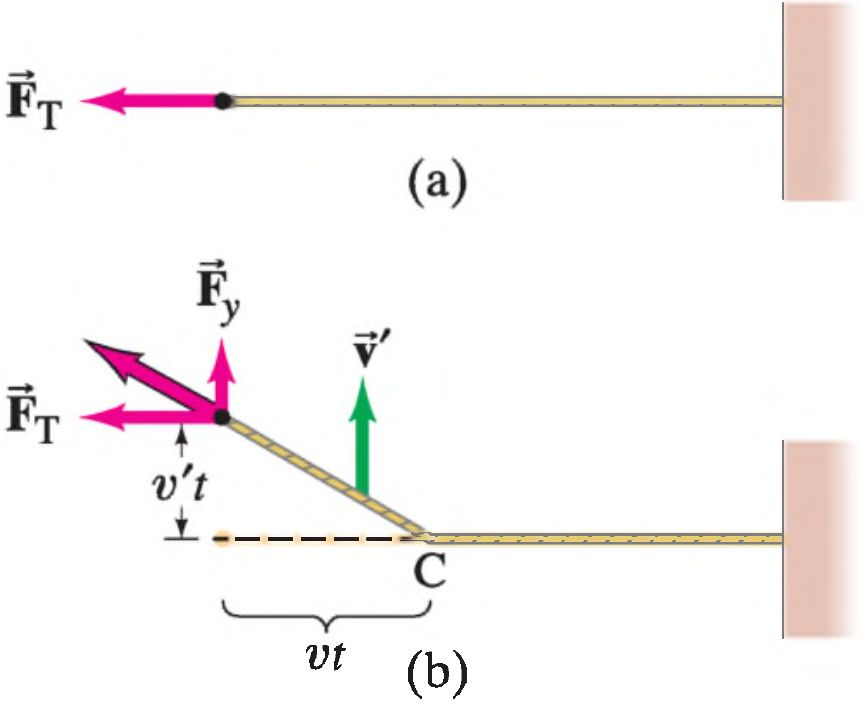
\includegraphics[height=1.5in]{images4/6.jpg}
\end{center}

  \pause
Small vertical displacement ($v't\ll vt$)
\pause
\begin{equation*}
\frac{F_y}{F_T}=\frac{v't}{vt}=\frac{v'}{v}
\end{equation*}
\pause
   \column{2.in}

Impulse:

 \begin{equation*}
F_y t=\Delta P'=\Delta mv'
\end{equation*}
\pause
\begin{equation*}
\Delta m=\mu x=\mu vt
\end{equation*}
\pause
\begin{equation*}
\rightarrow F_y t=\mu vtv' \rightarrow \frac{v'}{v}F_T=\mu vv'
\end{equation*}
\pause

\begin{equation}
\rightarrow v=\sqrt{\frac{F_T}{\mu}}
\end{equation}

   \end{columns}



  \end{frame}



%%%%%%%%%%%%%%%%%%%%%%%%%%%%%%%%%%%%%%%%%%%%%%%%%%%%%%%%%%%%%%%

\begin{frame}
\frametitle{Speed of transverse Waves}

In general...

\pause
\begin{equation*}
 v=\sqrt{\frac{elastic~force~factor}{inertia~factor}}
\end{equation*}
\pause
\vspace{2mm}

Longitudinal wave traveling down a long solid rod $ \rightarrow v=\sqrt{\frac{E}{\rho}}$

\pause
\vspace{2mm}
Longitudinal wave traveling in a liquid or gas $ \rightarrow v=\sqrt{\frac{B}{\rho}}$

\pause
\vspace{4mm}
Where, $E$ and $B$ are the elastic and bulk modulus, respectively.

  \end{frame}


%%%%%%%%%%%%%%%%%%%%%%%%%%%%%%%%%%%%%%%%%%%%%%%%%%%%%%%%%%%%%%%
\subsection{Energy transported by a wave}
\begin{frame}
\textcolor{mypink1}{Energy Transported by a Wave}
\pause
\vspace{4mm}


As a wave passes, each particle has an energy
\pause

\vspace{4mm}


\begin{equation}
 E=\frac{1}{2} k A^2\pause=\frac{1}{2} \omega^2 mA^2\pause= 2\pi^2 m\mathit{f}^2A^2
\end{equation}

\pause

\vspace{4mm}

For three-dimensional waves traveling in an elastic medium, $m=\rho V$, and $V=S\ell$ and $\ell=vt$:

\pause
  \begin{center}
  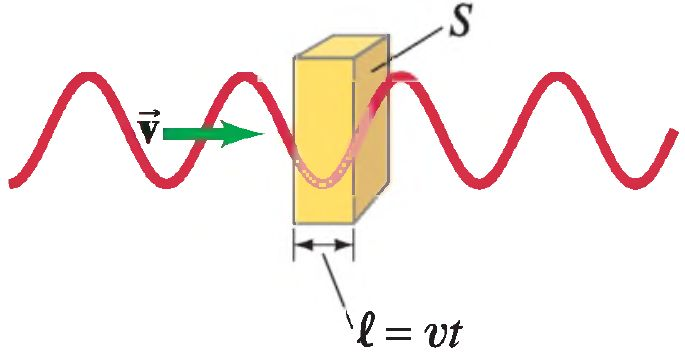
\includegraphics[height=0.8in]{images4/7.jpg}
\end{center}


  \end{frame}

%%%%%%%%%%%%%%%%%%%%%%%%%%%%%%%%%%%%%%%%%%%%%%%%%%%%%%%%%%%%%%%

\begin{frame}
Then, the energy is

\begin{equation}
E=2\pi^2\rho S v t f^2A^2
\end{equation}

\textit{The energy transported by a
wave is proportional to the square of the amplitude, and to the square o f the
frequency}.
\vspace{2mm}

\pause

The average rate of energy transferred is the average power P:

\pause

\begin{equation}
\overline P=\frac{E}{t}
\end{equation}


\end{frame}
%%%%%%%%%%%%%%%%%%%%%%%%%%%%%%%%%%%%%%%%%%%%%%%%%%%%%%%%%%%%%%%



\begin{frame}


The \textbf{ intensity}, $I$, of a wave is defined as the average power transferred
across unit area perpendicular to the direction of energy flow:

\pause

\begin{equation}
I= \frac{\overline P}{S}=\frac{E}{tS}=2\pi^2\rho  v f^2A^2
\end{equation}
\end{frame}
%%%%%%%%%%%%%%%%%%%%%%%%%%%%%%%%%%%%%%%%%%%%%%%%%%%%%%%%%%%%%%%


\begin{frame}
\frametitle{Point source in an isotropic medium}



   \begin{columns}[c]
   \column{2in}  % slides are 3in high by 5in wide
  
\pause

 \begin{center}
  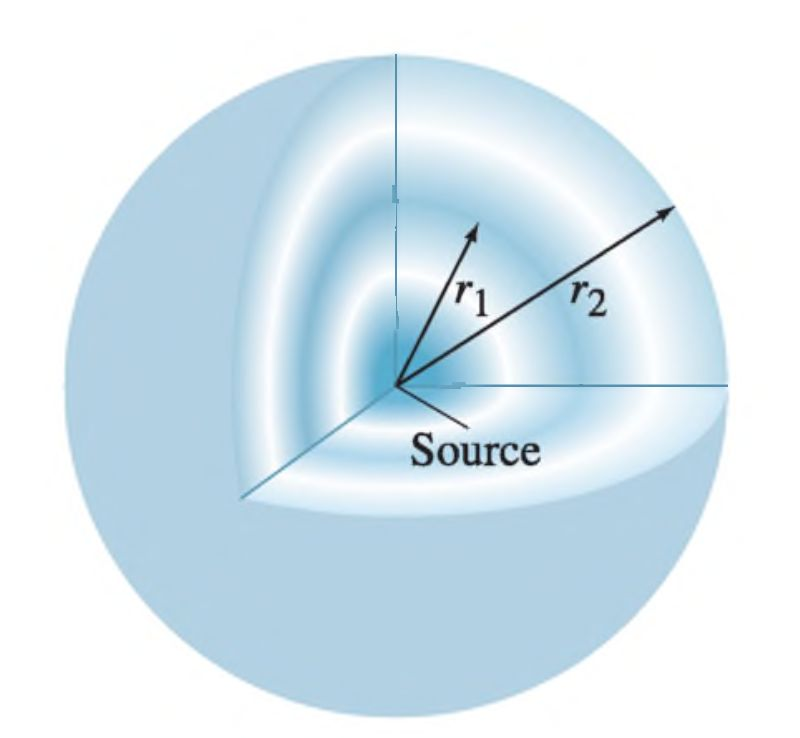
\includegraphics[height=1.2in]{images4/8.jpg}
\end{center}

   \column{2.4in}

\pause


If the medium is isotropic, the wave from a point source is
a spherical wave, the intensity is,

\pause

\begin{equation}
I=\frac{\overline P}{S}=\frac{\overline P}{4\pi r^2}
\end{equation}


   \end{columns}

\pause

If the power output P is constant $\rightarrow I\propto \frac{1}{r^2}$
\vspace{2mm}


  \end{frame}

  %%%%%%%%%%%%%%%%%%%%%%%%%%%%%%%%%%%%%%%%%%%%%%%%%%%%%%%%%%%%%%%


\begin{frame}
  \frametitle{Point source in an isotropic medium}
  
  
  
     \begin{columns}[c]
     \column{2in}  % slides are 3in high by 5in wide
    
  \pause
  
   \begin{center}
    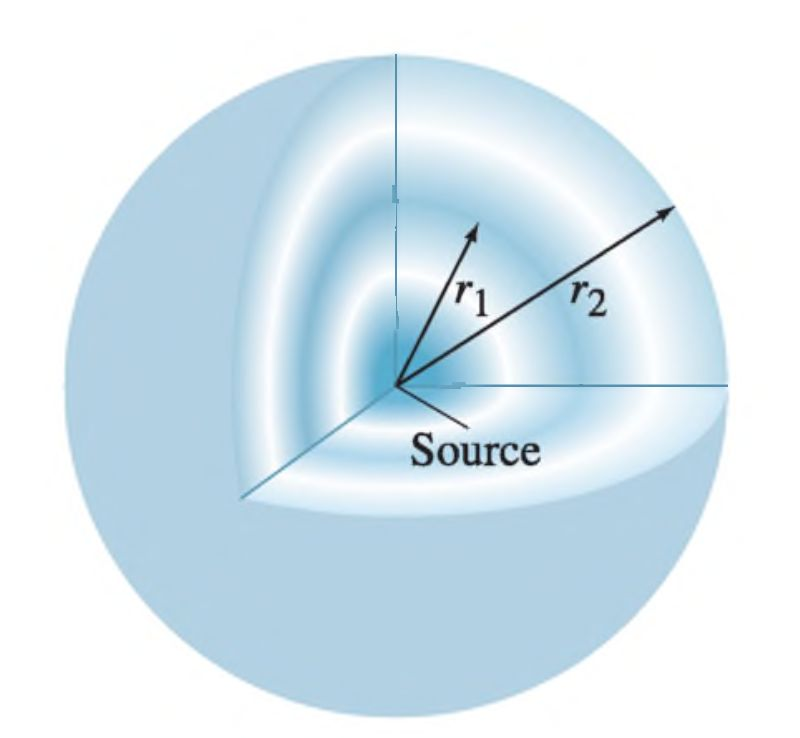
\includegraphics[height=1.2in]{images4/8.jpg}
  \end{center}
  
     \column{2.4in}
  
 

  
  When the distance doubles, then the intensity is
  reduced to $1/4$. The amplitude of a wave also decreases with distance,
  
  \pause
  
  \begin{equation}
  A\propto \frac{1}{r}
  \end{equation}
  
  \pause
  
  wave is twice as far from the source $\rightarrow$ amplitude is half as large.
  
\end{columns}
    \end{frame}

%%%%%%%%%%%%%%%%%%%%%%%%%%%%%%%%%%%%%%%%%%%%%%%%%%%%%%%%%%%%%%%
\subsection{Mathematical description of a Wave}

\begin{frame}


Suppose that at $t=0$, the wave shape is,

\pause
\begin{equation*}
D(x)=Asin\frac{2\pi}{\lambda}x, \pause ~~ \textcolor{mypink1}{ displacement~ of ~the ~wave ~at ~point ~x}
\end{equation*}

\pause
 If the wave is moving to the right, with speed $v$, then,

\pause

\begin{equation}
D(x,t)=Asin\big[\frac{2\pi}{\lambda}(x-vt)\big]
\end{equation}

\pause

 \begin{center}
  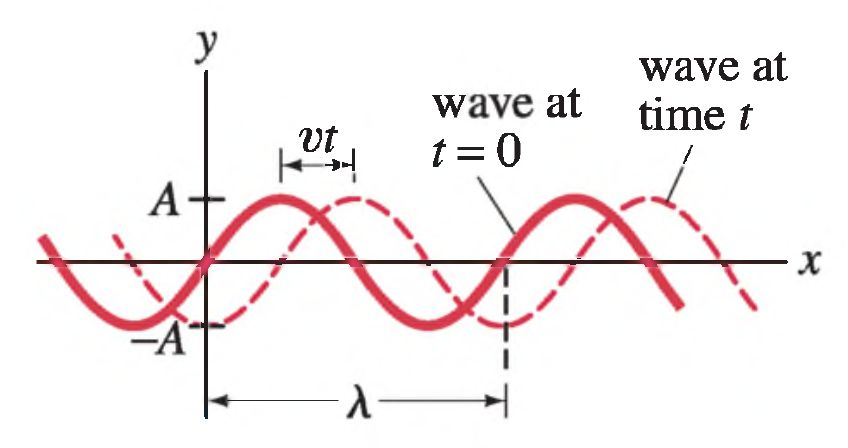
\includegraphics[height=1.2in]{images4/9.jpg}
\end{center}



  \end{frame}

%%%%%%%%%%%%%%%%%%%%%%%%%%%%%%%%%%%%%%%%%%%%%%%%%%%%%%%%%%%%%%%
\begin{frame}


We can write the expression of $D(x,t) $ as,



\begin{equation}
D(x,t)=Asin(\frac{2\pi}{\lambda}x-\frac{2\pi}{\lambda}vt)
\end{equation}





  \end{frame}

%%%%%%%%%%%%%%%%%%%%%%%%%%%%%%%%%%%%%%%%%%%%%%%%%%%%%%%%%%%%%%%
\begin{frame}


We can write the expression of $D(x,t) $ as,

\pause

\begin{equation}
D(x,t)=Asin(\frac{2\pi}{\lambda}x-\frac{2\pi}{\lambda}\underbrace{v}_{\textcolor{mypink1}{\lambda/T}}t)=Asin(\frac{2\pi}{\lambda}x-\frac{2\pi}{T}t)
\end{equation}



\pause


\begin{equation}
\rightarrow D(x,t)=Asin(kx-\omega t)
\end{equation}

\pause

\begin{itemize}
  \item \textcolor{mypink1}{$k\pause=\frac{2\pi}{\lambda}\pause\rightarrow$  \textbf{wave number}}\pause
  \item \textcolor{mypink1}{$(kx-\omega t) \pause\rightarrow$ phase }\pause
  \item \textcolor{mypink1}{$v \pause\rightarrow$ phase velocity}
\end{itemize}



\pause
\begin{equation}
\boxed{v=\frac{2\pi}{k}\frac{\omega}{2\pi}=\frac{\omega}{k}}
\end{equation}

  \end{frame}


%%%%%%%%%%%%%%%%%%%%%%%%%%%%%%%%%%%%%%%%%%%%%%%%%%%%%%%%%%%%%%%
\begin{frame}


Wave traveling to the left:

\pause

\begin{equation}
D(x,t)=Asin(kx+\omega t)
\end{equation}

\pause

The argument of the sine can also contain a phase $\phi$ determined by the value of $D$ at $x=0,~t=0$.
  \end{frame}


%%%%%%%%%%%%%%%%%%%%%%%%%%%%%%%%%%%%%%%%%%%%%%%%%%%%%%%%%%%%%%%
\subsection{The Wave Equation}

\begin{frame}


\frametitle{The Wave Equation}


Apply Newton  to a segment of a string $\pause \rightarrow$ Obtain Wave equation

\pause
\vspace{6mm}

We assume:

\pause
\vspace{2mm}



\begin{itemize}
\item The amplitude of the wave is small compared to the wavelength.

\pause
\item The tension in the string does not vary during a vibration.
\end{itemize}


  \end{frame}



%%%%%%%%%%%%%%%%%%%%%%%%%%%%%%%%%%%%%%%%%%%%%%%%%%%%%%%%%%%%%%%


\begin{frame}
  \frametitle{The Wave Equation}
  
  
  
     \begin{columns}[c]
     \column{2in}  % slides are 3in high by 5in wide
     \begin{center}
    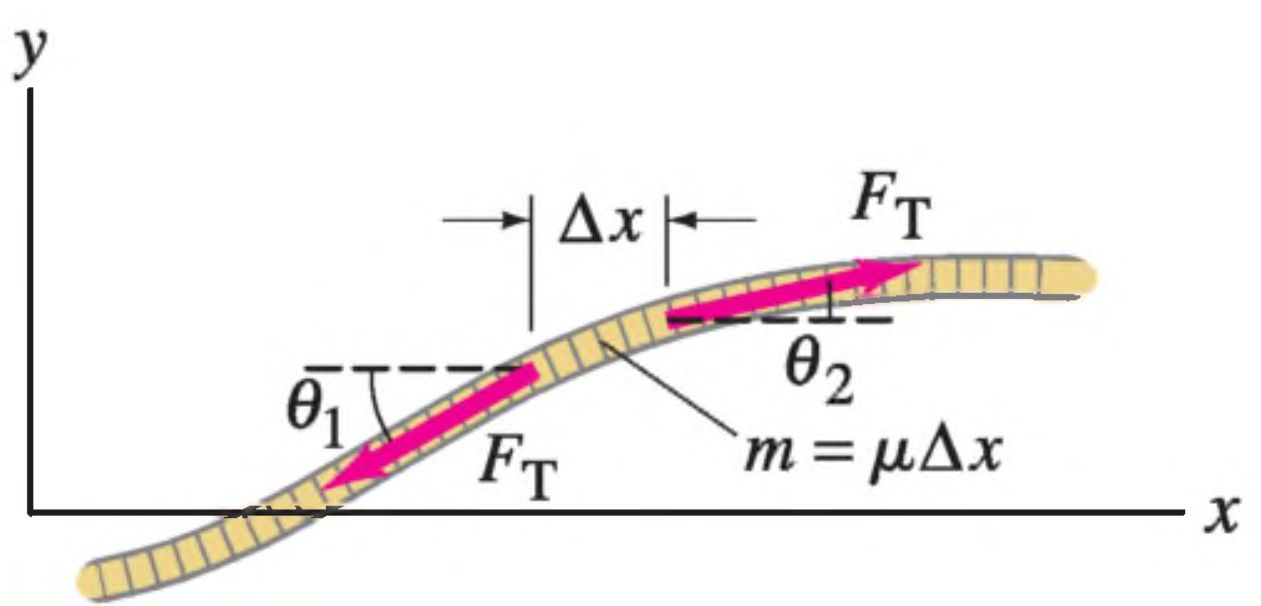
\includegraphics[height=1.in]{images4/10.jpg}
  \end{center}
  
  
  
  
  
  
     \column{2.5in}
  
     \pause
     \begin{equation*}
     Newton \rightarrow \sum F_y=ma_y
      \end{equation*}
      
      \pause
  
  
      \begin{equation*}
        F_Tsin\theta_2-F_Tsin\theta_1= m a
        \end{equation*}
  

  

  
  
  
  
     \end{columns}
  
  
  
  
  
  
  
  
  
    \end{frame}

%%%%%%%%%%%%%%%%%%%%%%%%%%%%%%%%%%%%%%%%%%%%%%%%%%%%%%%%%%%%%%%


\begin{frame}
\frametitle{The Wave Equation}



   \begin{columns}[c]
   \column{2in}  % slides are 3in high by 5in wide
   \begin{center}
  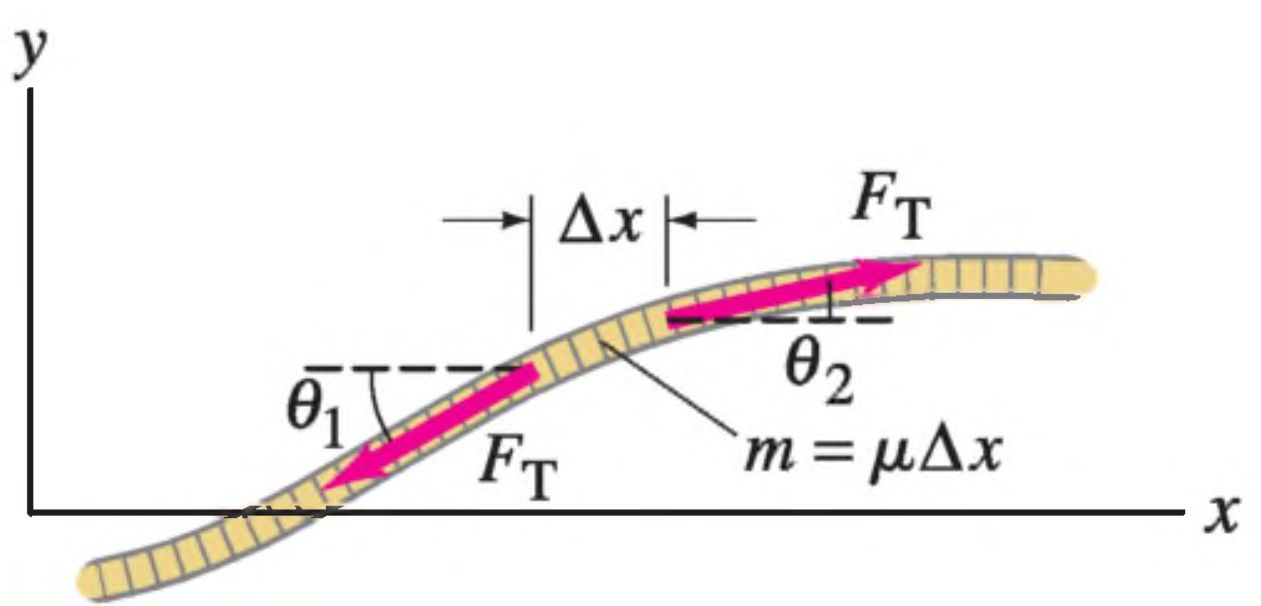
\includegraphics[height=1.in]{images4/10.jpg}
\end{center}






   \column{2.5in}

  
   \begin{equation*}
   Newton \rightarrow \sum F_y=ma_y
    \end{equation*}

 
      
\begin{equation*}
F_Tsin\theta_2-F_Tsin\theta_1=(\textcolor{mypink1}{\mu\Delta x})\textcolor{mypink1}{\frac{\partial^2 D}{\partial t^2}}
\end{equation*}


\pause

\begin{equation*}
 sin\theta\approx tan\theta=\frac{\partial D}{\partial x}=S
\end{equation*}

\end{columns}

\end{frame}







%%%%%%%%%%%%%%%%%%%%%%%%%%%%%%%%%%%%%%%%%%%%%%%%%%%%%%%%%%%%%%%


\begin{frame}
\frametitle{The Wave Equation}


Then, our equation becomes,

\pause

\begin{equation*}
F_T(S_2-S_1)=\mu \Delta x\frac{\partial^2D}{\partial^2 t}
\end{equation*}

Or..

\pause

\begin{equation*}
F_T\frac{\Delta S}{\Delta x}=\mu \frac{\partial^2D}{\partial^2 t}
\end{equation*}

\pause



\begin{equation*}
  (\Delta x \rightarrow 0) ~~\pause \rightarrow \pause \lim_{x\to 0} F_T\frac{\Delta S}{\Delta x}=F_T\frac{\partial}{\partial x}\left(\frac{\partial D}{\partial x}\right)=F_T\frac{\partial^2D}{\partial x^2}
\end{equation*}
\pause




  \end{frame}






%%%%%%%%%%%%%%%%%%%%%%%%%%%%%%%%%%%%%%%%%%%%%%%%%%%%%%%%%%%%%%%


\begin{frame}
\frametitle{The Wave Equation}




\begin{equation}
\rightarrow \frac{\partial^2D}{\partial x^2}=\frac{\mu}{F_T} \frac{\partial^2D}{\partial^2 t}
\end{equation}


\pause

\begin{equation*}
\rightarrow v=\sqrt{\frac{F_T}{\mu}}
\end{equation*}


  \end{frame}


%%%%%%%%%%%%%%%%%%%%%%%%%%%%%%%%%%%%%%%%%%%%%%%%%%%%%%%%%%%%%%%


\begin{frame}
\frametitle{The Wave Equation}



Then,


\begin{equation}
\boxed{\frac{\partial^2D}{\partial x^2}=\frac{1}{v^2} \frac{\partial^2D}{\partial^2 t}}
\end{equation}

\pause

\vspace{3mm}

\textcolor{mypink1}{This is the \textbf{one-dimensional} wave equation, and it can describe not only small
amplitude waves on a stretched string, but also small amplitude longitudinal waves
in gases, liquids, and elastic solids.}

  \end{frame}

%%%%%%%%%%%%%%%%%%%%%%%%%%%%%%%%%%%%%%%%%%%%%%%%%%%%%%%%%%%%%%%

\section{Superposition Principle}

\begin{frame}
\frametitle{Superposition Principle}

If $D_1$ and $D_2$ are solutions of 

\begin{equation*}
\frac{\partial^2D}{\partial x^2}=\frac{1}{v^2} \frac{\partial^2D}{\partial^2 t}
\end{equation*}

\vspace{3mm}

Then,  $D_1+D_2$ is  a solution.
\vspace{3mm}

\pause

When two or more waves pass through the same region of space at the same time,
 the displacement is the vector sum of the separate displacements.


  \end{frame}





%%%%%%%%%%%%%%%%%%%%%%%%%%%%%%%%%%%%%%%%%%%%%%%%%%%%%%%%%%%%%%%


\begin{frame}
\frametitle{Superposition Principle}



   \begin{columns}[c]
   \column{2in}  % slides are 3in high by 5in wide
  
Sum of three  sinusoidal Waves $\pause \rightarrow$ it is not sinusoidal.

   \column{2in}


  \begin{center}
  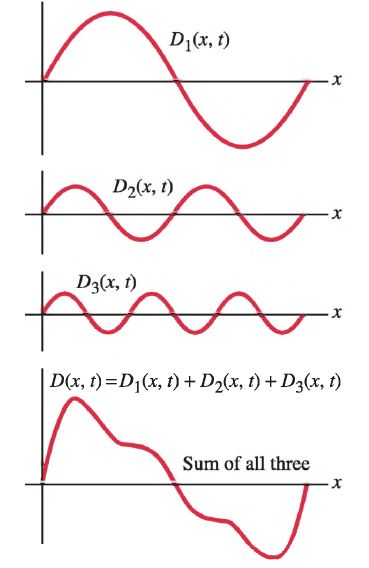
\includegraphics[height=2.in]{images4/11.jpg}
\end{center}


   \end{columns}




  \end{frame}


%%%%%%%%%%%%%%%%%%%%%%%%%%%%%%%%%%%%%%%%%%%%%%%%%%%%%%%%%%%%%%%


\begin{frame}
  \frametitle{Superposition Principle}
  
  The shape changes if the velocity of the waves depends on the frequency. $\pause \rightarrow$ Dispersion
  
  \begin{center}
    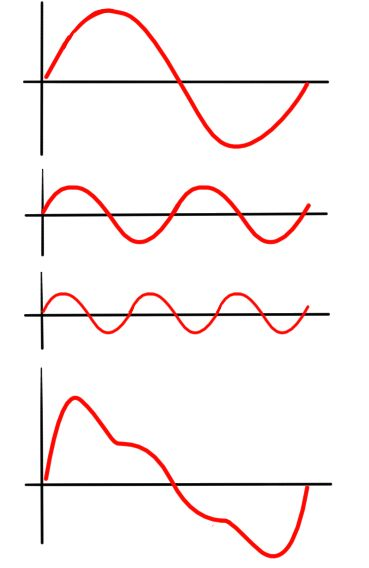
\includegraphics[height=2.in]{images4/dispersion1.jpg}
  \end{center}
  
  \end{frame}
  
  
  %%%%%%%%%%%%%%%%%%%%%%%%%%%%%%%%%%%%%%%%%%%%%%%%%%%%%%%%%%%%%%%
  
  
  \begin{frame}
  \frametitle{Superposition Principle}
  
Dispersion

    \begin{center}
    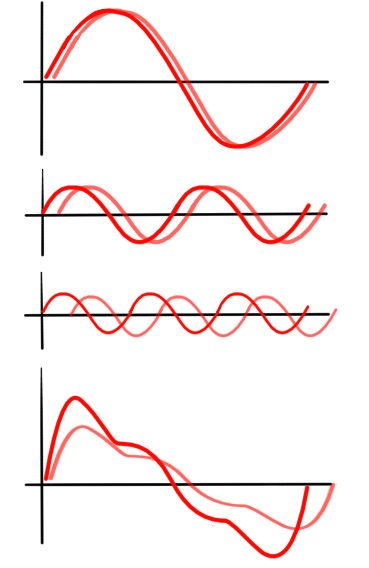
\includegraphics[height=2.in]{images4/dispersion2.jpg}
  \end{center}
  
  
    \end{frame}
%%%%%%%%%%%%%%%%%%%%%%%%%%%%%%%%%%%%%%%%%%%%%%%%%%%%%%%%%%%%%%%


\begin{frame}
\frametitle{Superposition Principle}

\textcolor{mypink1}{Fourier's Theorem:}

\vspace{4mm}
\pause

\textcolor{mypink1}{Any complex periodic wave $=$  sum of simple sinusoidal waves}

\pause

\vspace{3mm}
If the wave is not periodic, the sum becomes an integral (called a Fourier integral).


  \end{frame}


%%%%%%%%%%%%%%%%%%%%%%%%%%%%%%%%%%%%%%%%%%%%%%%%%%%%%%%%%%%%%%%

\begin{frame}
\frametitle{Superposition Principle}



\begin{equation}
f(x)=\frac{a_0}{2}+\sum^{\infty}_{n=1} a_n cos\left(\frac{2n\pi x}{P}\right)+\sum^{\infty}_{n=1} b_n sin\left(\frac{2n\pi x}{P}\right)
\end{equation}

\pause


where $f(x)$  integrable  in the interval $(-P/2,P/2)$ 
\begin{equation}
  a_0=\frac{2}{P}\int^{P/2}_{-P/2}f(x)dx
  \end{equation}

  
\begin{equation}
a_n=\frac{2}{P}\int^{P/2}_{-P/2}f(x)cos\left(\frac{2n\pi x}{P}\right)dx
\end{equation}

\begin{equation}
b_n=\frac{2}{P}\int^{P/2}_{-P/2}f(x)sin\left(\frac{2n\pi x}{P}\right)dx
\end{equation}



  \end{frame}










% %%%%%%%%%%%%%%%%%%%%%%%%%%%%%%%%%%%%%%%%%%%%%%%%%%%%%%%%%%%%%%%


% \begin{frame}
% \frametitle{Reflection and transmission }




% For reflection of a two- or three-dimensional plane wave,
% the angle that the incoming or incident wave makes with the reflecting surface is
% equal to the angle made by the reflected wave. This is the\textbf{ law of reflection}:

% \vspace{3mm}

% \textbf{the angle of reflection equals the angle of incidence.}


%   \begin{center}
%   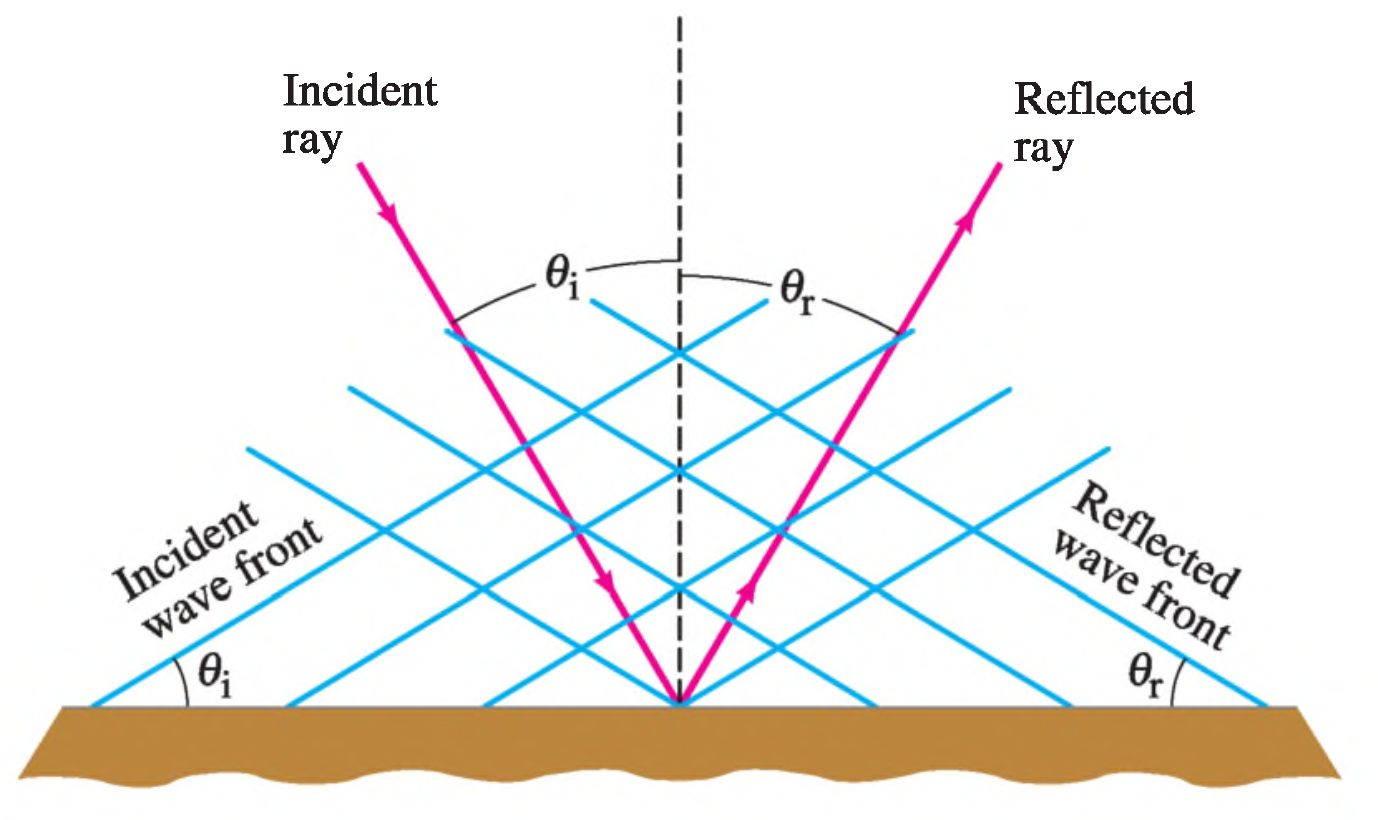
\includegraphics[height=1.5in]{images4/14.jpg}
% \end{center}

%   \end{frame}







%%%%%%%%%%%%%%%%%%%%%%%%%%%%%%%%%%%%%%%%%%%%%%%%%%%%%%%%%%%%%%%

\subsection{Interference}
\begin{frame}
\frametitle{Interference }




Interference: two waves pass through the same region of space at the same time. .


\pause
\begin{itemize}
\item \textbf{Destructive Interference} the two waves have opposite displacements and they
add to zero. 

\pause
\item \textbf{Constructive Interference} they produce a resultant displacement that is greater than the
displacement of either separate pulse,
\end{itemize}


  \end{frame}






%%%%%%%%%%%%%%%%%%%%%%%%%%%%%%%%%%%%%%%%%%%%%%%%%%%%%%%%%%%%%%%

\begin{frame}
\frametitle{Interference }

Example two pulses in a cord:




  \begin{center}
  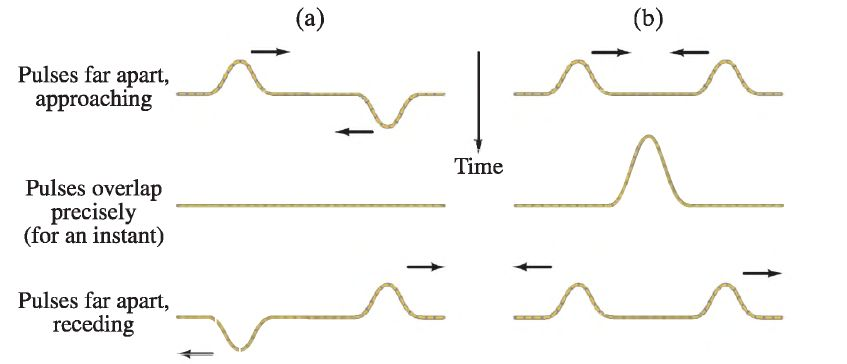
\includegraphics[height=1.8in]{images4/15.jpg}
\end{center}





  \end{frame}





%%%%%%%%%%%%%%%%%%%%%%%%%%%%%%%%%%%%%%%%%%%%%%%%%%%%%%%%%%%%%%%

\begin{frame}
  \frametitle{Interference }
  
  The interference pattern of two equal waves can be constructive (waves is phase, phase $0$ degree), destructive (out of phase, phase $180$ degree), partially destructive
  (other angles or different amplitudes).
  
  
  
  
  
  
  
    \begin{center}
    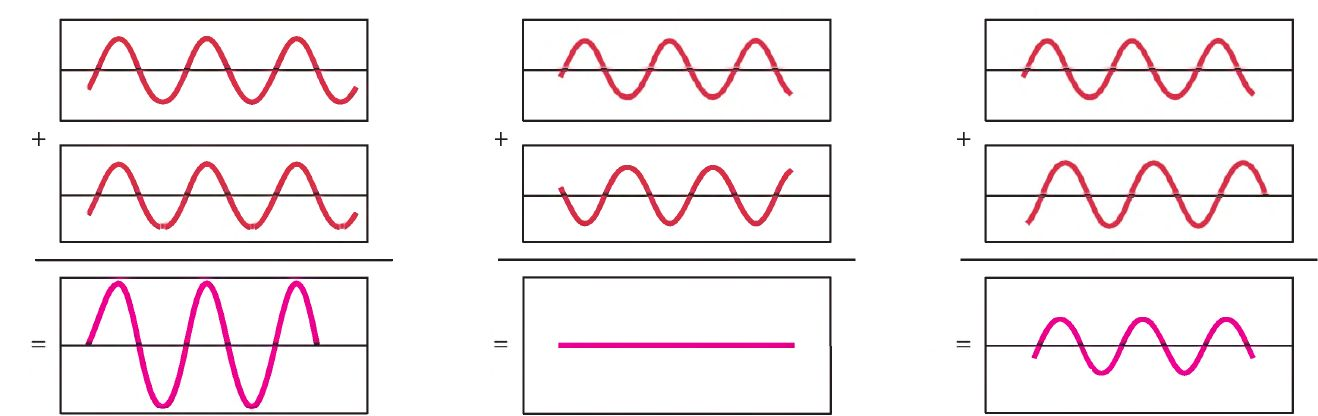
\includegraphics[height=1.4in]{images4/17.jpg}
  \end{center}
  
  
  







    \end{frame}

%%%%%%%%%%%%%%%%%%%%%%%%%%%%%%%%%%%%%%%%%%%%%%%%%%%%%%%%%%%%%%%

\subsection{Reflection and transmission}
\begin{frame}
\frametitle{Reflection and transmission }

What happens when  a wave strikes an obstacle, or comes to the end of the medium in which it is
traveling?


  \end{frame}





%%%%%%%%%%%%%%%%%%%%%%%%%%%%%%%%%%%%%%%%%%%%%%%%%%%%%%%%%%%%%%%


\begin{frame}
\frametitle{Reflection and transmission }

\textcolor{mypink1}{Change of medium}

  \begin{center}
  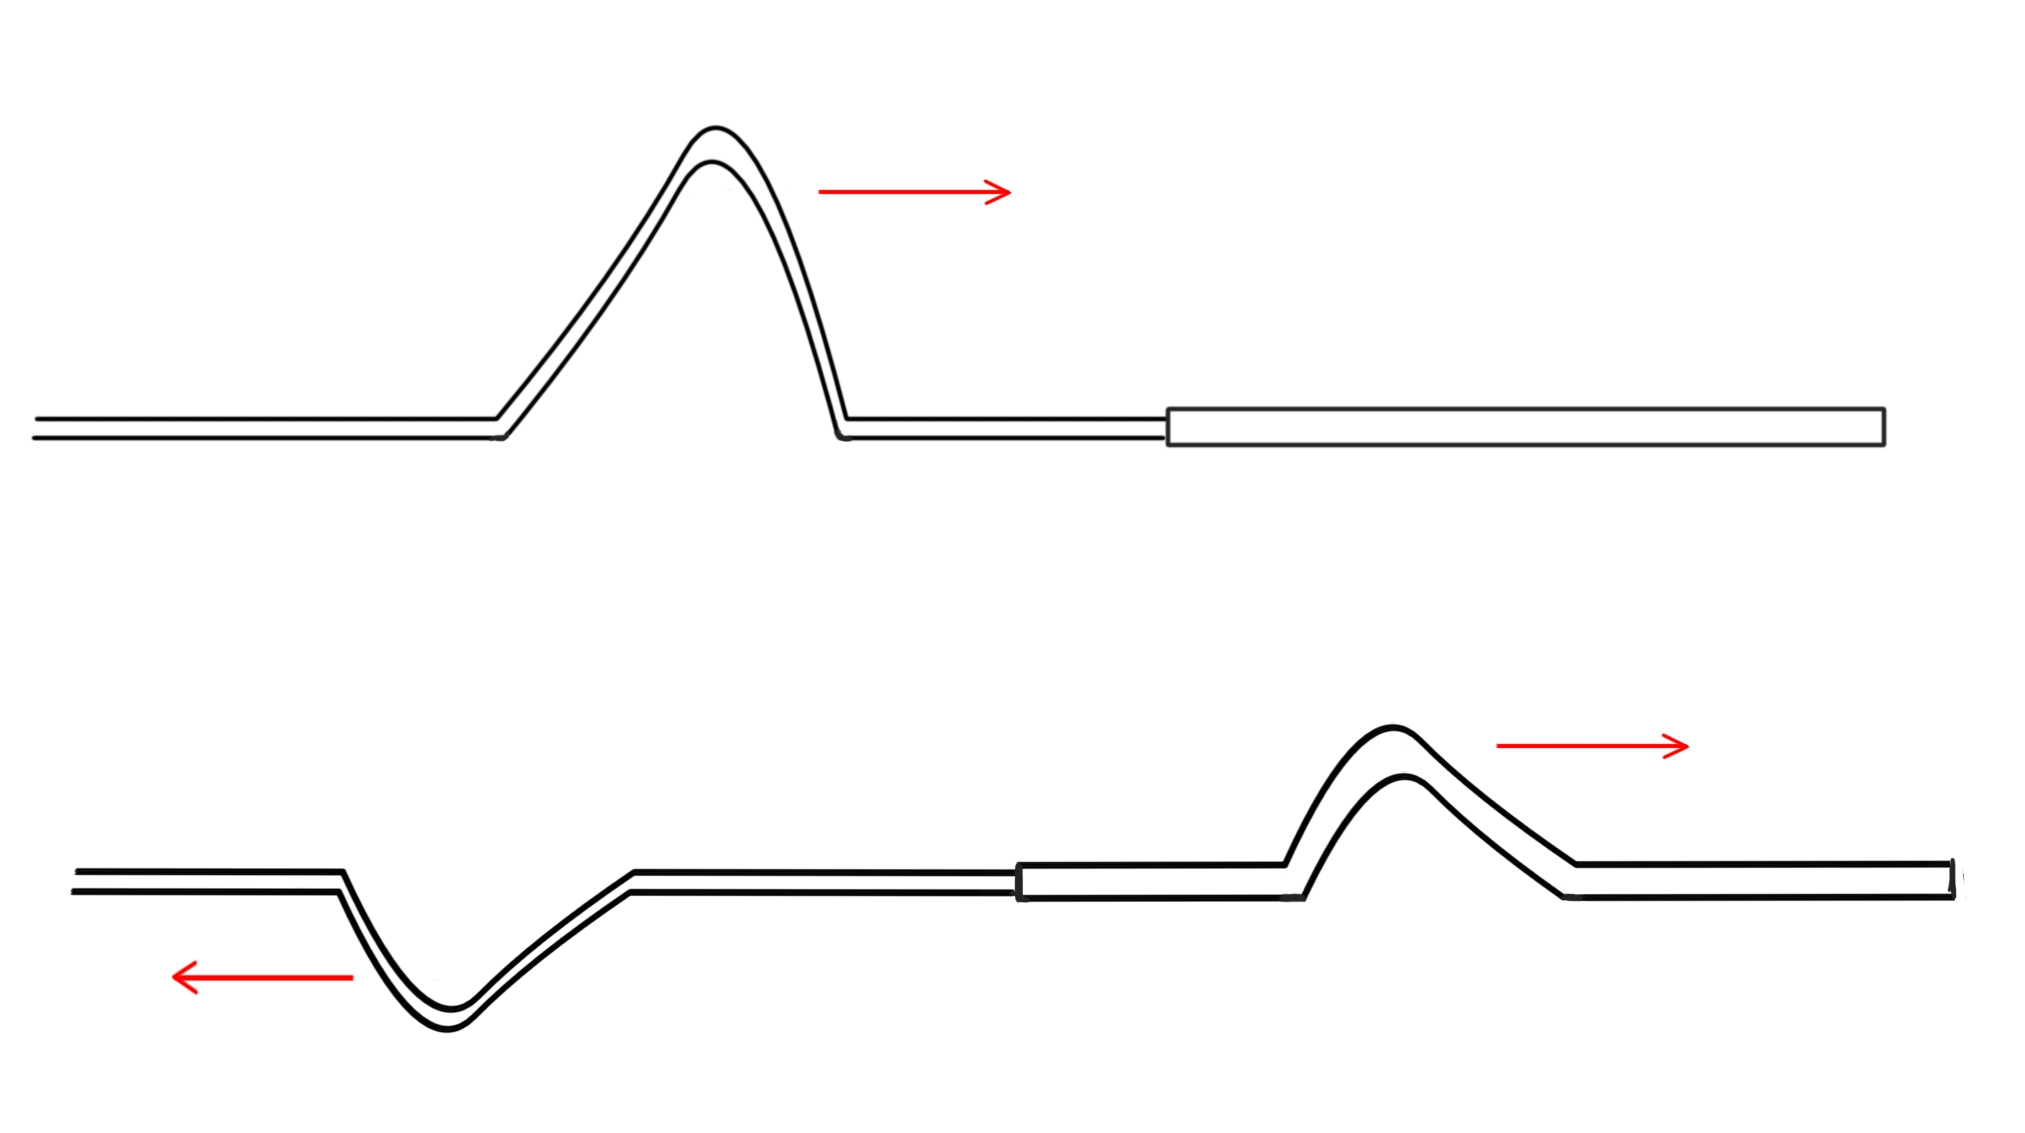
\includegraphics[height=2.in]{images4/reflection.jpg}
\end{center}



  \end{frame}



%%%%%%%%%%%%%%%%%%%%%%%%%%%%%%%%%%%%%%%%%%%%%%%%%%%%%%%%%%%%%%%


 \begin{frame}
 \frametitle{Reflection and transmission }

% Example:






%    \begin{columns}[c]
%    \column{2in}  % slides are 3in high by 5in wide


% A wave pulse traveling down a cord is reflected as shown in the figure. The
% reflected pulse returns inverted if the end of the cord is fixed; it
% returns right side up if the end is free.

  
%    \column{2in}

   \begin{center}
   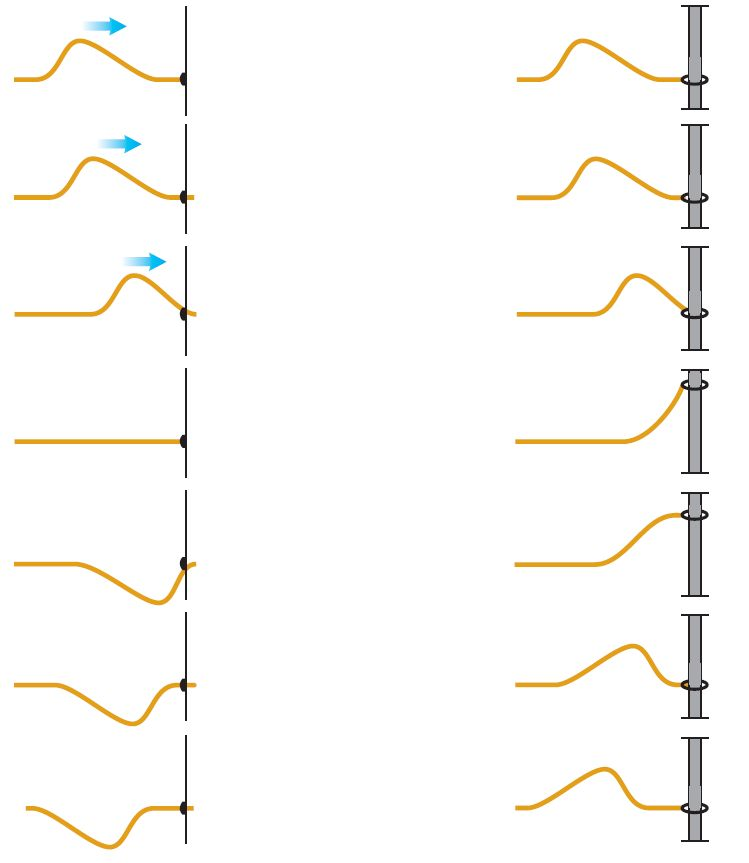
\includegraphics[height=2.4in]{images4/12.jpg}
 \end{center}

%    \end{columns}



  \end{frame}


%%%%%%%%%%%%%%%%%%%%%%%%%%%%%%%%%%%%%%%%%%%%%%%%%%%%%%%%%%%%%%%

\subsection{Standing waves  }
%%%%%%%%%%%%%%%%%%%%%%%%%%%%%%%%%%%%%%%%%%%%%%%%%%%%%%%%%%%%%%%






\begin{frame}
\frametitle{Resonance}

String fixed at its two ends, \pause What happens when the string is pocked?


  \begin{center}
  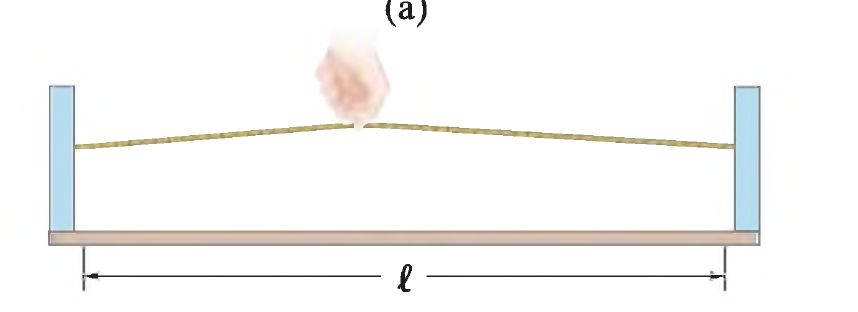
\includegraphics[height=1.4in]{images4/19.jpg}
\end{center}

\pause

The initial pulse generates two traveling waves that are  reflected in both extremes. 
  \end{frame}

%%%%%%%%%%%%%%%%%%%%%%%%%%%%%%%%%%%%%%%%%%%%%%%%%%%%%%%%%%%%%%%


\begin{frame}
\frametitle{Resonance}



\begin{equation*}
D(x,t)=D_1(x,t)+D_2(x,t)
\end{equation*}

\pause

Imagine that the string is pocked periodically, with a sinusoidal function
\pause


\begin{equation*}
D_1(x,t)=Asin(kx-\omega t),~D_2(x,t)=Asin(kx+\omega t)
\end{equation*}


\begin{equation}
\rightarrow \boxed{D(x,t)=2Asin(kx)cos(\omega t)} \pause ~~\textcolor{mypink1}{Standing~Wave}
\end{equation}


  \end{frame}


%%%%%%%%%%%%%%%%%%%%%%%%%%%%%%%%%%%%%%%%%%%%%%%%%%%%%%%%%%%%%%%



\begin{frame}
\frametitle{Resonance}

If the string is fixed at its two ends,

\begin{equation*}
D(x=0,t)=D(x=\ell,t)=0
\end{equation*}
then,

\begin{equation}
 k\ell=n\pi \rightarrow k=\frac{ n\pi}{\ell}
\end{equation}

\begin{equation}
  \lambda_n=\frac{2\ell}{n},~n=1~,2~,3,...
  \end{equation}

\end{frame}


%%%%%%%%%%%%%%%%%%%%%%%%%%%%%%%%%%%%%%%%%%%%%%%%%%%%%%%%%%%%%%%



\begin{frame}
\frametitle{Resonance}


All particles of the string vibrate with
the same frequency:

\begin{equation}
f_n=\frac{v}{\lambda_n}
\end{equation}

\pause

\begin{equation}
\rightarrow f_n=n \frac{v}{2\ell}\pause = \boxed{\frac{n}{2\ell} \textcolor{mypink1}{ \sqrt{\frac{F_T}{\mu}}}}
\end{equation}

\pause



\textcolor{mypink1}{\textbf{Fundamental frequency}:} $n=1\rightarrow f_1$
  
\vspace{3mm}

\textcolor{mypink1}{\textbf{Harmonics}} $\rightarrow  f_n$



  \end{frame}

%%%%%%%%%%%%%%%%%%%%%%%%%%%%%%%%%%%%%%%%%%%%%%%%%%%%%%%%%%%%%%%



\begin{frame}
  \frametitle{Resonance}

The amplitude of the motion depends on $x$,
  
  
  \begin{equation*}
  amplitude=2Asin(kx)
  \end{equation*}
  
  The amplitude has a maximum, equal to $2A$, when
  
  \begin{equation}
   kx=\frac{(2n+1)\pi}{2} \rightarrow x=\frac{(2 n+1)\pi}{k}
  \end{equation}
  

  
  
    \end{frame}






%%%%%%%%%%%%%%%%%%%%%%%%%%%%%%%%%%%%%%%%%%%%%%%%%%%%%%%%%%%%%%%

\begin{frame}
\frametitle{Resonance}




The frequencies at which standing waves are produced are the \textbf{natural frequencies}
or \textbf{resonant frequencies} of the cord.



When a  string is pocked, only standing waves corresponding to resonant frequencies persist for long.



  \end{frame}







%%%%%%%%%%%%%%%%%%%%%%%%%%%%%%%%%%%%%%%%%%%%%%%%%%%%%%%%%%%%%%%







\begin{frame}
\frametitle{Resonance}


\begin{center}
  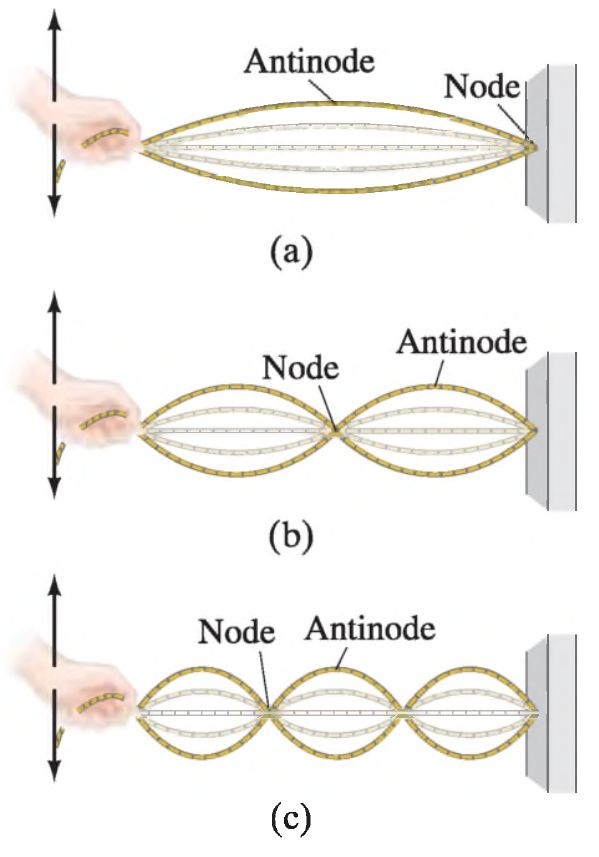
\includegraphics[height=2.4in]{images4/18.jpg}
\end{center}








  \end{frame}








%%%%%%%%%%%%%%%%%%%%%%%%%%%%%%%%%%%%%%%%%%%%%%%%%%%%%%%%%%%%%%%


\begin{frame}
\frametitle{Resonance}



  \begin{center}
  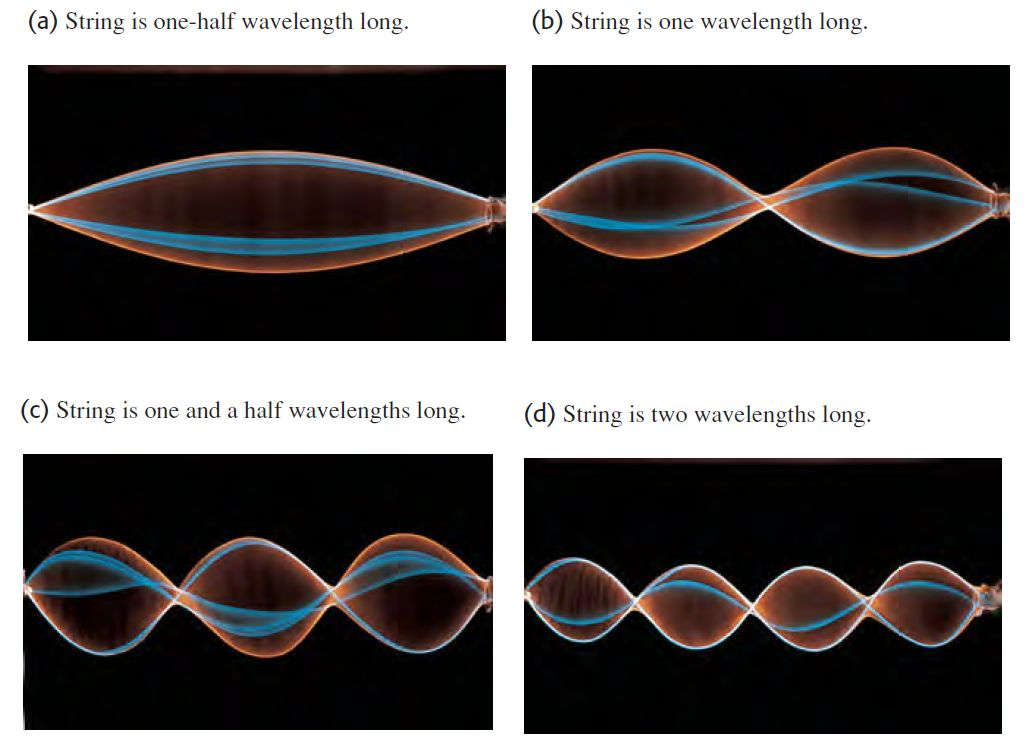
\includegraphics[height=2.4in]{images4/20.jpg}
\end{center}


  \end{frame}




%%%%%%%%%%%%%%%%%%%%%%%%%%%%%%%%%%%%%%%%%%%%%%%%%%%%%%%%%%%%%%%

\begin{frame}
\frametitle{Resonance}


\begin{itemize}
  \item  The term “standing” wave is also meaningful from the point of view
  of energy. Since the string is at rest at the nodes, no energy flows past these points.
  Hence the energy is not transmitted down the string but “stands” in place in the string.\pause
  \item Standing waves are produced not only on strings, but on any object that is
  struck, such as a drum membrane or an object made of metal or wood.
  
\end{itemize}






  \end{frame}





%%%%%%%%%%%%%%%%%%%%%%%%%%%%%%%%%%%%%%%%%%%%%%%%%%%%%%%%%%%%%%%

\begin{frame}
\frametitle{Questions}

\begin{enumerate}

\item Describe how you could estimate the speed of water waves
across the surface of a pond.
\pause
\item Will any function of $(x- v t)$ represent a
wave motion?
\pause


\item When a standing wave exists on a string, the vibrations of
incident and reflected waves cancel at the nodes. Does this
mean that energy was destroyed? 

\pause

\item Can the amplitude of the standing waves  be
greater than the amplitude of the vibrations that cause them
(up and down motion of the hand)?


\end{enumerate}

  \end{frame}
































%%%%%%%%%%%%%%%%%%%%%%%%%%%%%%%%%%%%%%%%%%%%%%%%%%%%%%%%%%%%%%%
 \end{document}
%%%%%%%%%%%%%%%%%%%%%%%%%%%%%%%%%%%%%%%%%%%%%%%%%%%%%%%%%%%%%%%